\section{实验结果}\label{sec:results}

\subsection{训练过程分析}

\begin{figure}[!htp]
	\begin{minipage}{0.5\textwidth}
		\centering
		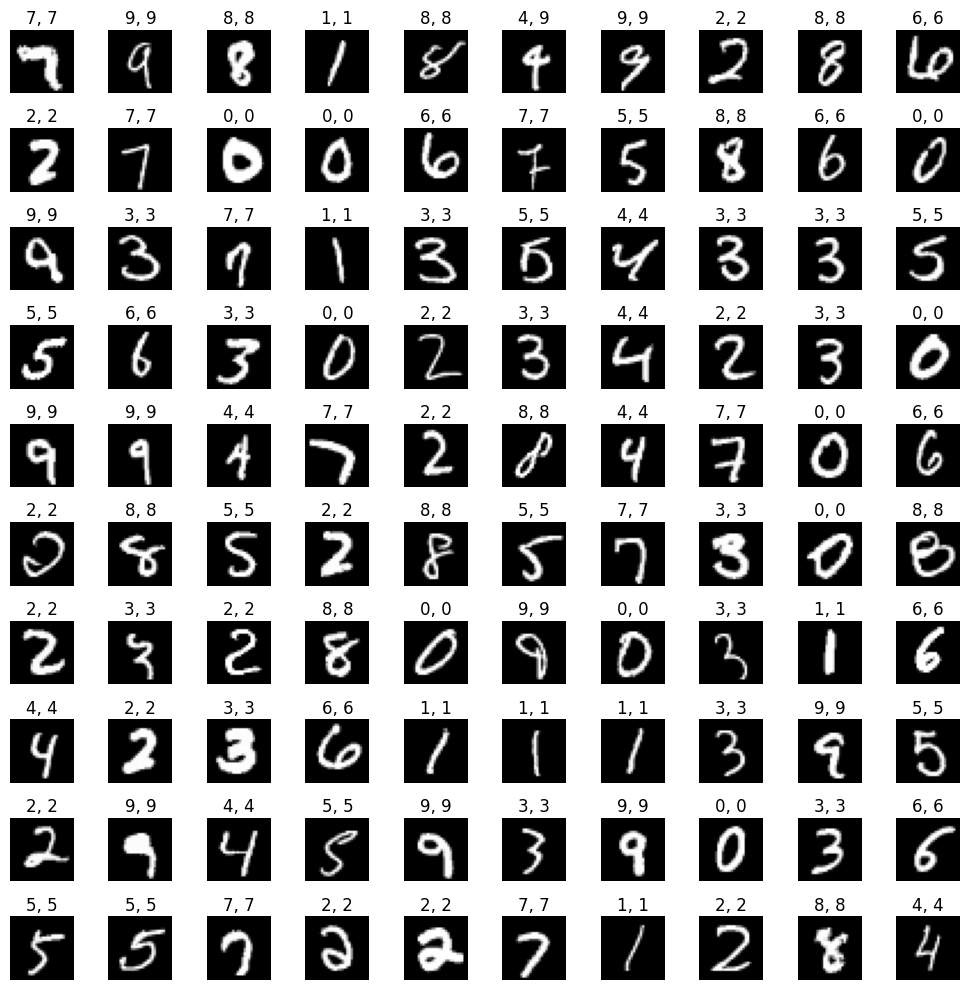
\includegraphics[height=0.25\textheight]{figures/dataset_predictions}
		\caption{部分手写数字数据集标签与预测结果}
	\end{minipage}\hfill
	\begin{minipage}{0.5\textwidth}
		\centering
		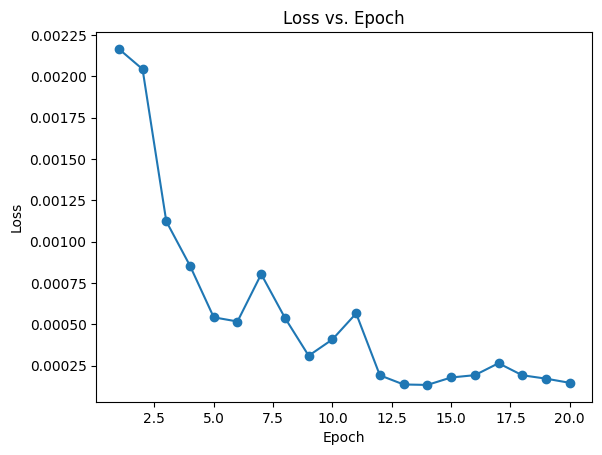
\includegraphics[height=0.25\textheight]{figures/loss_curve}
		\caption{CNN模型训练损失随epoch变化曲线}
	\end{minipage}
\end{figure}

我们观察到模型在训练过程中表现出了良好的收敛性和稳定性。随着训练的进行,平均训练损失逐渐减小,这表明模型对训练数据的拟合效果逐渐提高。在每个epoch内,小批量训练损失也呈现逐渐减小的趋势。这种逐步减小的损失趋势证明了模型在不断优化参数以适应训练数据的过程中的有效性。值得注意的是,随着训练的进行,损失的下降速度逐渐减缓,这表明模型在后续训练中对数据的拟合程度逐渐增加,进一步证实了模型的收敛性。

我们观察到在epoch在6到12之间时,训练过程中的平均损失出现了小范围的波动。这种现象可能是由于多种因素相互作用所致。学习率的调整可能导致模型参数更新速度的变化,引起损失的波动。数据批量的影响也是一个重要因素,特定批量数据的特性可能会对模型训练产生影响。此外,模型复杂性以及随机性也可能在一定程度上影响了损失的变化。这种小范围的损失波动通常被认为是正常的,只要整体的训练损失仍然在下降趋势中。

\subsection{测试结果分析}

在测试集上,我们评估了模型的性能,获得了99.19\%的准确率。这说明模型在未见过的数据上具有很好的泛化能力,能够有效地识别手写数字。此外,我们计算了模型在测试集上的平均损失,结果为0.00058,这表明模型的预测结果与真实标签之间的差距很小。综合考虑准确率和损失值,我们可以得出结论,模型在测试集上表现出了出色的性能,验证了其在实际应用中的有效性和稳定性。需要指出的是,许多被模型错误预测的例子,即使对人类来说也可能难以准确识别。因此,我们的模型在实践中的表现非常出色。

\begin{figure}[htbp]
  \centering
  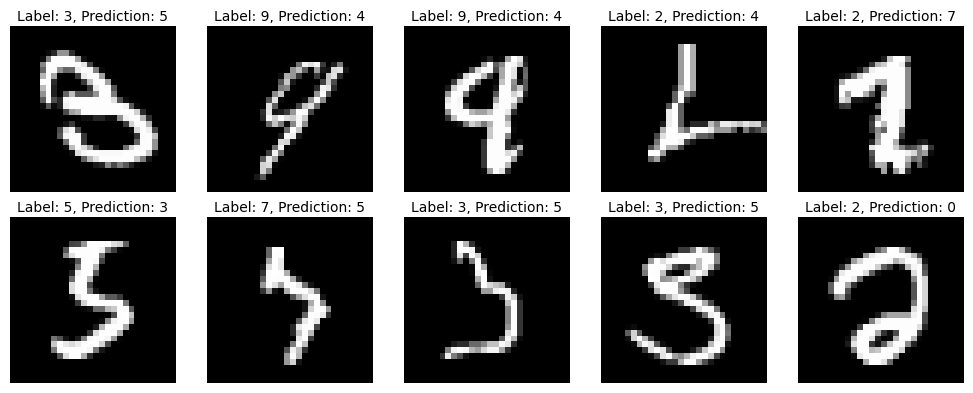
\includegraphics[width=0.5\textwidth]{figures/dataset_mispredictions}
  \caption{部分手写数字数据集标签与错误的预测结果}
\end{figure}